\documentclass[sigconf]{acmart}

\usepackage{graphicx}
\usepackage{hyperref}
\usepackage{todonotes}

\usepackage{endfloat}
\renewcommand{\efloatseparator}{\mbox{}} % no new page between figures

\usepackage{booktabs} % For formal tables

\settopmatter{printacmref=false} % Removes citation information below abstract
\renewcommand\footnotetextcopyrightpermission[1]{} % removes footnote with conference information in first column
\pagestyle{plain} % removes running headers

\newcommand{\TODO}[1]{\todo[inline]{#1}}

\begin{document}
\title{IoT Application Using MQTT and Raspberry Pi Robot Car}

\author{Arnav Arnav}
\affiliation{%
  \institution{Indiana University Bloomington}
  \city{Bloomington} 
  \state{Indiana} 
  \postcode{47408}
  \country{USA}
}
\email{aarnav@iu.edu}


% The default list of authors is too long for headers}
%\renewcommand{\shortauthors}{G. v. Laszewski}


\begin{abstract}
As the number of connected edge devices increases there is a need for fast 
comunication between these devices, and to analyse the data collected by
these devices, which is made possible by the use of a scalable lightweight 
communicatoin protocol such as MQTT, which is easy to use, data agnostic, and 
application independent.
We look at one such appllication of the protocol, to control a robot car remotely,
over wireless network, navigating with the help of a raspberry pi camera on the car.

\end{abstract}

\keywords{i523, HID201, Edge Computing, Raspberry Pi, MQTT, Robot Car, IoT}


\maketitle


\section{Introduction}

As the number of edge devices increases, and sensor networks become more and more common in Internet of Things (IoT) applications, the need arises to allow these resource constrained devices to communicate with each other in a power efficient and secure manner. In many cases these devices may not be able to process trafitional HTTP requests efficiently, and as the number of devices increases, sending an HTTP request to each of the dvices in order to get data may not be efficient \cite{mqtt-vs-http}\cite{hivemq-website}.

Message Queue Telemetry Transport (MQTT) is a lightweight  machine to machine (M2M) messaging protocol, that uses a client/server based publish/subscribe model and is ideal for IoT applications. The protocol has been designed on top of TCP/IP protocol for us in situations where network bandwidth ad available memory are limited \cite{mqtt-wiki}\cite{mqtt-official}.
The Eclipse Paho Project curently provides suport for MQTT \cite{eclipse-mosquitto}. MQTT clients are available for various languages like Python, C, and Lua.

We look at one such application here that uses MQTT for communication between a raspberry pi and a desktop. The raspberry pi controls the stepper motors of the robot car according to the message it recieves over mqtt, and drives the car accordigly. another program running on the raspberry pi uses the rasperry pi onboard camera to capture pictures and send them back to the desktop to helo in navigation. Thus we create a simple robot car that can be used remotely for monitoring purposes. The robot car can be controlled from anywhere in the world, as long as both the controlling device (desktop) and the raspberry pi can conect to the MQTT broker.

We can use multiple such cars and controlling devices to control the cars independently or from a commn device to drive mltiple cars together, thus controlling a swarm of cars. As these cars may be using different platforms like raspberry pi or arduino, Using MQTT allows us to write the controller program independent of the subscriber programs running on the different robot cars and even in different languages. All that is needed to control a car is that the subscriber can understand the messages sent by the controller.

\section{Related Work}
There have been many edge computing applications that involve robot cars or swarm of cars.

\cite{sentdex-pi-car} provides an example of a raspberry pi car that uses distance sensor, and face detection on the raspberry pi 2. The car is controlled over wifi and is built using the GoPiGo robot car kit \cite{gopigo}

Zheng Wang used raspberry pi in \cite{self-driving-rc-car} to build a sophisticated self driving car that can detect stop signs and traffic signals and drive appropriately on a small test track. The car has a camera and a distance sensor that stream data to a TCP server running on a desktop. The system uses Haar Cascades provided in opencv to detect objects like stop signs and traffic signals and a trained neural network which uses the image to predigt the direction in which the car should move. The distance is calculated using the image from the raspberry pi camera with the help of a monocular vision method proposed by Chu, Ji, Guo, Li and Wang in 2004 \cite{monocular}.
 
As the part of Eclipse IoT open challenge \cite{bitreactive} built a robot car that is controlled using the Constrained Application Protocol (CoAP) which snaps images and communicates the images over MQTT

OpenHAB provides a vendor neutral platform that allows users to integrate vatious home automation systema and provides an application interface to control those devices \cite{openhab}. It allows integration of various devices with MQTT.

The FloodNet project at University of Southampton \cite{floodnet} aims at ``providing a pervasive, continuous embedded monitoring presence''. The system is intelligent and obtains `` environmental self-awreness and resilience to ensure robust transmission of data'', ensuring data quality and allowing exploration of environments in new ways. The project uses MQTT for communicating data from the sensors on field to visualization and simulation applications.

As a part of IBM's Extreme Blue projects, Say it Sign it \cite{SiSi} is a sophisticated, innovative speech to sign language translation system. The application uses speech recognition and renders an avatar that signs the corresponding words in British sign Language, using MQTT and microbroker for communication.


\section{Technologies and Hardware}
The project uses MQTT to communicate between a controller running on a desktop and a raspberry pi that drives the robot car with the help of stepper motors. We describe these technologies in detail.

\subsection{MQTT}
MQTT works via a publish-subscribe model that contains 3 entities: (1) a
publisher, that sends a message, (2) a broker, that maintains queue of all
messages based on topics and (3) multiple subscribers that subscribe to
various topics they are interested in \cite{how-mqtt-works}.

This allows for decoupling of functionality at various levels. The
publisher and subscriber do not need to be close to each other and do
not need to know each others identity. They need only to know the
broker, as the publisher and the subscribers do not have to be running
either at the same time nor on the same hardware
\cite{hivemq-details}.

MQTT implements a hierarchy of topics that are related
to all messages. These topics are recognised by strings separated by a
forward-slash ( / ), where each part represents a different topic
level. This is a common model introduced in file systems but also in
internet URLs. 

A topic looks therefore as follows: {\em topic-level0/topic-level1/topic-level2}.

All subscribers subscribe to different topics via the broker.
Subscribing to {\em topic-level0} allows the subscriber to receive all
messages that are associated with topics that start with {\em
topic-level0}.

This is different from traditional message queues as the message is
forwarded to multiple subscribers, and allows for a more flexible
approach with the help of topics \cite{hivemq-details}. The basic
steps in an MQTT client application include connecting to the broker,
subscribing to some topics, waiting for messages and performing the
appropriate action when a certain message is received
\cite{mqtt-wiki}.

MQTT allows the publisher and subscriber to respond to messages withthe help of callbacks that are executed on different events ,in a non-blocking manner. The paho-mqtt package for python provides callbacks methods like on-connect(), on-message() and on-disconnect(), which are fired when
the connection to the broker is complete, a message is received from
the broker, and when the client is disconnected from the broker
respectively. These methods are used in conjunction with the
loop-start() and loop-end() methods which start and end an
asynchronous loop that listens for these events and fires the relevant
callbacks, allowing the clients to perform other tasks
\cite{python-paho-mqtt}.

MQTT has been designed to be flexible and options are provided to
easily change the quality of service (QoS) as required by the
application. Three basic levels of QoS are supported by the protocol,
Atmost-once (QoS level 0), Atleast-once (QoS level 1) and Atmost-once
(QoS level 2) \cite{hivemq-qos}\cite{python-paho-mqtt}.

The QoS level of 0 can be used in applications where some dropped
messages may not affect the application. Under this QoS level, the
broker forwards a message to the subscribers only once and does not
wait for any acknowledgement \cite{hivemq-qos}
\cite{python-paho-mqtt}.

The QoS level of 1 can be used in situations where the delivery of all
messages is important and the subscriber can handle duplicate
messages. Here the broker keeps on resending the message to a
subscriber after a certain timeout until the first acknowledgement is
received. A QoS level of 2 should be used in cases where all messages
must be delivered and no duplicate messages should be allowed. In this
case the broker sets up a handshake with the subscriber to check for
its availability before sending the message \cite{hivemq-qos}
\cite{python-paho-mqtt}.

The MQTT specification uses TCP/IP to deliver the messaged to the
subscribers, but it does not provide any form of security by default
to make is useful for resource constrained IoT devices. ``It allows
the use of username and password for authentication, but by default
this information is sent as plain text over the network, making it
susceptible to man-in-the middle attacks''
\cite{iot-design-mqtt-security} \cite{mqtt-sec-ssl}. Therefore, in
sensitive applications some form of additional security measures are
recommended which may include network layer security with the use of
Virtual Private Networks (VPNs), Transport Layer Security, or
application layer security \cite{mqtt-sec-ssl}.

Transport Layer Security (TLS) and Secure Sockets Layer (SSL) are
cryptographic protocols that establish a the identity of the server
and client with the help of a handshake mechanism which uses trust
certificates to establish identities before encrypted communication
can take place \cite{ibm-mqtt-security}. If the handshake is not
completed for some reason, the connection is not established and no
messages are exchanged \cite{mqtt-sec-ssl}. ``Most MQTT brokers
provide an option to use TLS instead of plain TCP and port 8883 has
been standardized for secured MQTT connections''
\cite{iot-design-mqtt-security}.

Using TLS/SSL security however comes at an additional cost. If the
connections are short-lived then most of the time can be spent in the
handshake itself, which may take up few kilobytes of bandwidth. In
case the connections are short-lived, temporary session IDs and
session tickets can be used to resume a session instead of repeating
the handshake process. If the connections are long term, the overhead
of the handshake is negligible and TLS/SSL security should be used
\cite{iot-design-mqtt-security}\cite{mqtt-sec-ssl}.

Although MQTT protocol itself does not include authorization, many MQTT brokers
include authorization as an additional feature
\cite{ibm-mqtt-security}. OAuth2.0 uses JSON Web Tokens which contain
information about the token ans the user and are signed by a trusted
authorization server \cite{hivemq-security-oauth}.

When connecting to the broker this token can be used to check whether
the client is authorised to connect at this time or not. Additionally
the same validations can be used when publishing or subscribing to the
broker. The broker may use a third party resource such as LDAP
(lightweight directory access protocol) to look up authorizations for
the client \cite{hivemq-security-oauth}. Since there can be a large
number of clients and it can become impractical to authorize everyone,
clients may be grouped and the authorizations may be checked for each
group \cite{ibm-mqtt-security}.

MQTT allows easy integration with other services, that have
been designed to process this data.

Apache storm is a distributed processing system that allows real time
processing of continuous data streams, much like Hadoop works for
batch processing \cite{apache-storm}. Apache storm can be easily
integrated with MQTT as shown in \cite{apache-storm-mqtt} to get real
time data streams and allow analytics and online machine learning in a
fault tolerant manner \citep{apache-storm-wiki}.

ELK stack (elastic-search, logstash and kibana) is an opensource
project designed for scalability which contains three main software
packages, the {\em elastic-search} search and analytics engine, {\em
  logstash} which is a data collection pipeline and {\em kibana} which
is a visualization dashboard \cite{elk-stack}. Data from an IoT
network can be collected, analysed and visualized easily with the help
of the ELK stack as shown in \cite{mqtt-elasticsearch-setup} and
\cite{kibana-mqtt-analysis}.

MQTT broker services can be utilized for enterprise and production
environments. EMQ (Erlang MQTT Broker) provides a highly scalable,
distributed and reliable MQTT broker that can be used in
enterprise-grade applications \cite{erlang-mqtt-broker}.


\subsection{Raspberry Pi}

The raspberry pi is a credit card sized development board that was developed by Eben Upton with the goal to crate a low cost device that can be used for education and prototypiing \cite{os-pi}. Since its creation the board has been adapted for various different projects by educators hobbyists and in the industry \cite{pi-official}. The board is developed as open hardware except for the Broadcom chip that controls the main components of the board, and most raspberry pi projects are available openly with detailed documentation.

The board's Broadcom system on chip consists of an ARM processor and it can be used just like a normal computer by connnecting a monitor, a keyboard and a mouse. The raspberry pi can communicate to other devices with the help of wifi and bluetooth and is capable of accessing the internet. All this put together makes the raspberry pi a very useful device \cite{pi-official}.

The raspberry pi comes in various models, Model A+, which is one of the smallest form factors, rasbperry pi2 Model B, raspberry pi3 Model B and Model B+ that have more gpio pins. The raspberry pi 3 Model B is the newest design and consists of on board wifi and bluetooth, eliminating the need to use usb wifi and bluetooth attachments. It has a 1.2 GHz ARM 8 microprocessor, 1 GB RAM, a dual core Videocore IV GPU, and 40 general purpose input and output (GPIO) pins. The board has an ethernet port and four USB ports and an HDMI port to connect to a monitor \cite{pi-compare}\cite{element-compare}.

The raspberry pi Zero is the deveopment board that has the smallest form factor. Even though the the raspberry pi zero includes no ehternet or USB ports, and does not come with GPIO pins soldered on, its small size and cost effectiveness make it extremely useful in applications such as IoT where space is constrained \cite{official-pi-zero}.

The raspberry pi uses a micro SD card to boot and various operating systems, that support the ARM architecture can be used. The most common operating systems are Raspbian, a derivative of the Debian linux, and Pidora, a derivative of Fedora. There are other operating systems cantered around using the raspberry pi for various purposes, like openELEC and RaspBMC, which make it easy to use raspberry pi as a multimedia center. For, users who want non-linux operating system, RISC OS may be a good choice. The raspberry pi foundation provides new users the opportunity to try out various operating systems with the help of their New Out  Of The Box Software (NOOBS), which allows the users to pick which operating system they want to use \cite{os-pi}.

Variuos different shields are available for the raspberry pi that make it simple to connect to various peripherals, and extend the functionality of the raspberry pi, such as the Grovepi shield, provided by Dexter Industries, which alows simple interface with may digital and analog sensors and actuators provided by Dexter.

\subsection{Stepper Motors}
Stepper motors are brushless motors that divide the complete rotation into a number of parts known as steps. The motor consists of electromagnetic coils and a rotating core that aligns itself according to the combined magnetic effect of the coils. The stepper motor can move from one step to another and remain in a single step based on which coils are turned on. The torque of the otor can be increased or decreased with the current supplied to the coils, and the speed of rotation can be controlled by setting the time interval between switching the coils on and off \cite{wiki-stepper}.

% how they work
Stepper motors can be controlled in various ways, dependng on the application. 
Figure \ref{f:stepper1} shows how a steppper motor with a resolution of 90 degrees can be made to complete one full rotation. In practice however, the resolution (the degrees moved at each step) of most stepper motors is much higher. The process mentioned in figure \ref{f:stepper1} is known as half stepping \cite{stepper1}.

\begin{figure}[!ht]
  \centering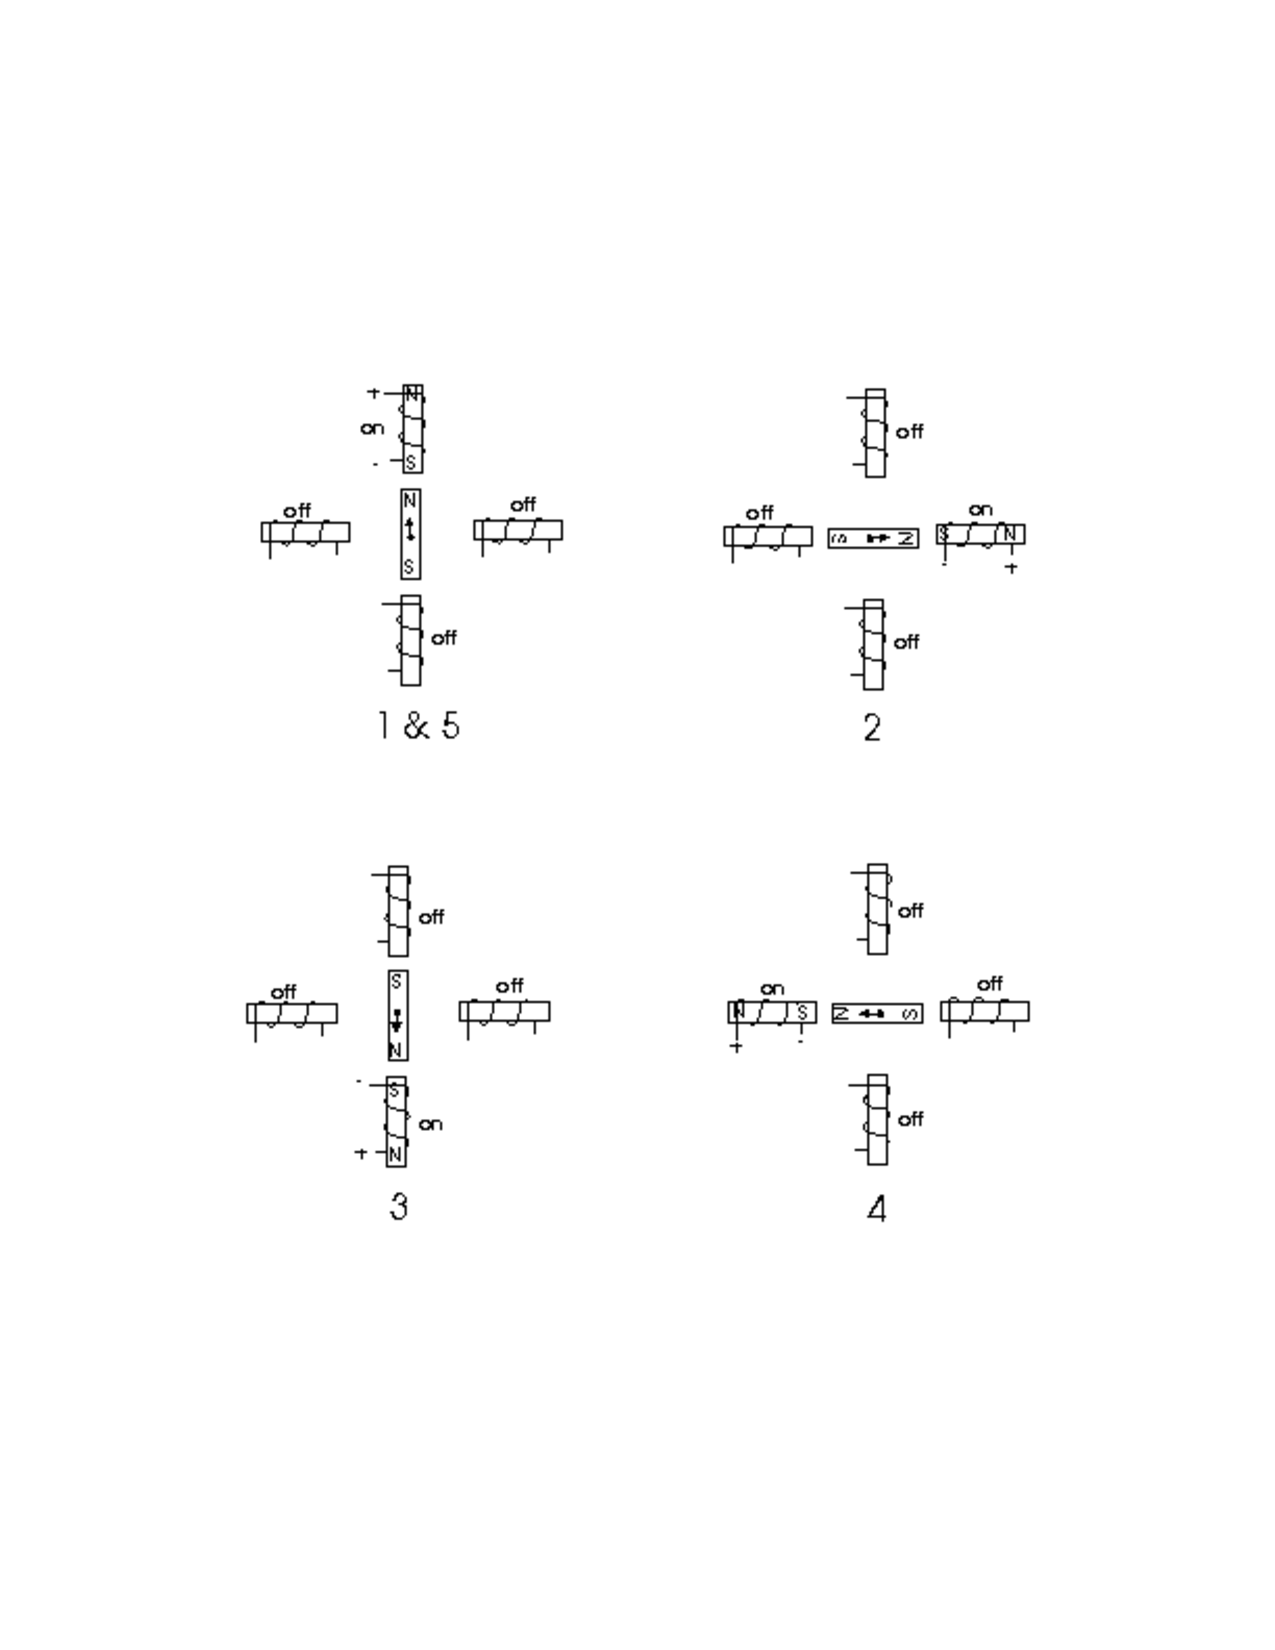
\includegraphics[width=\columnwidth]{images/stepper1.pdf}
  \caption{Working of a steper motor : Full stepping using one coil at a time \cite{stepper1}}\label{f:stepper1}
\end{figure}

In the above method, only one coil is turned on at a time. This can be improved upon to get a higher torque. To get a higher torque, two adjescent coils are turned on at the same time, as shown in figure \ref{f:stepper2}. This results in double the torque generated when using only one coil at a time \cite{stepper2}.

\begin{figure}[!ht]
  \centering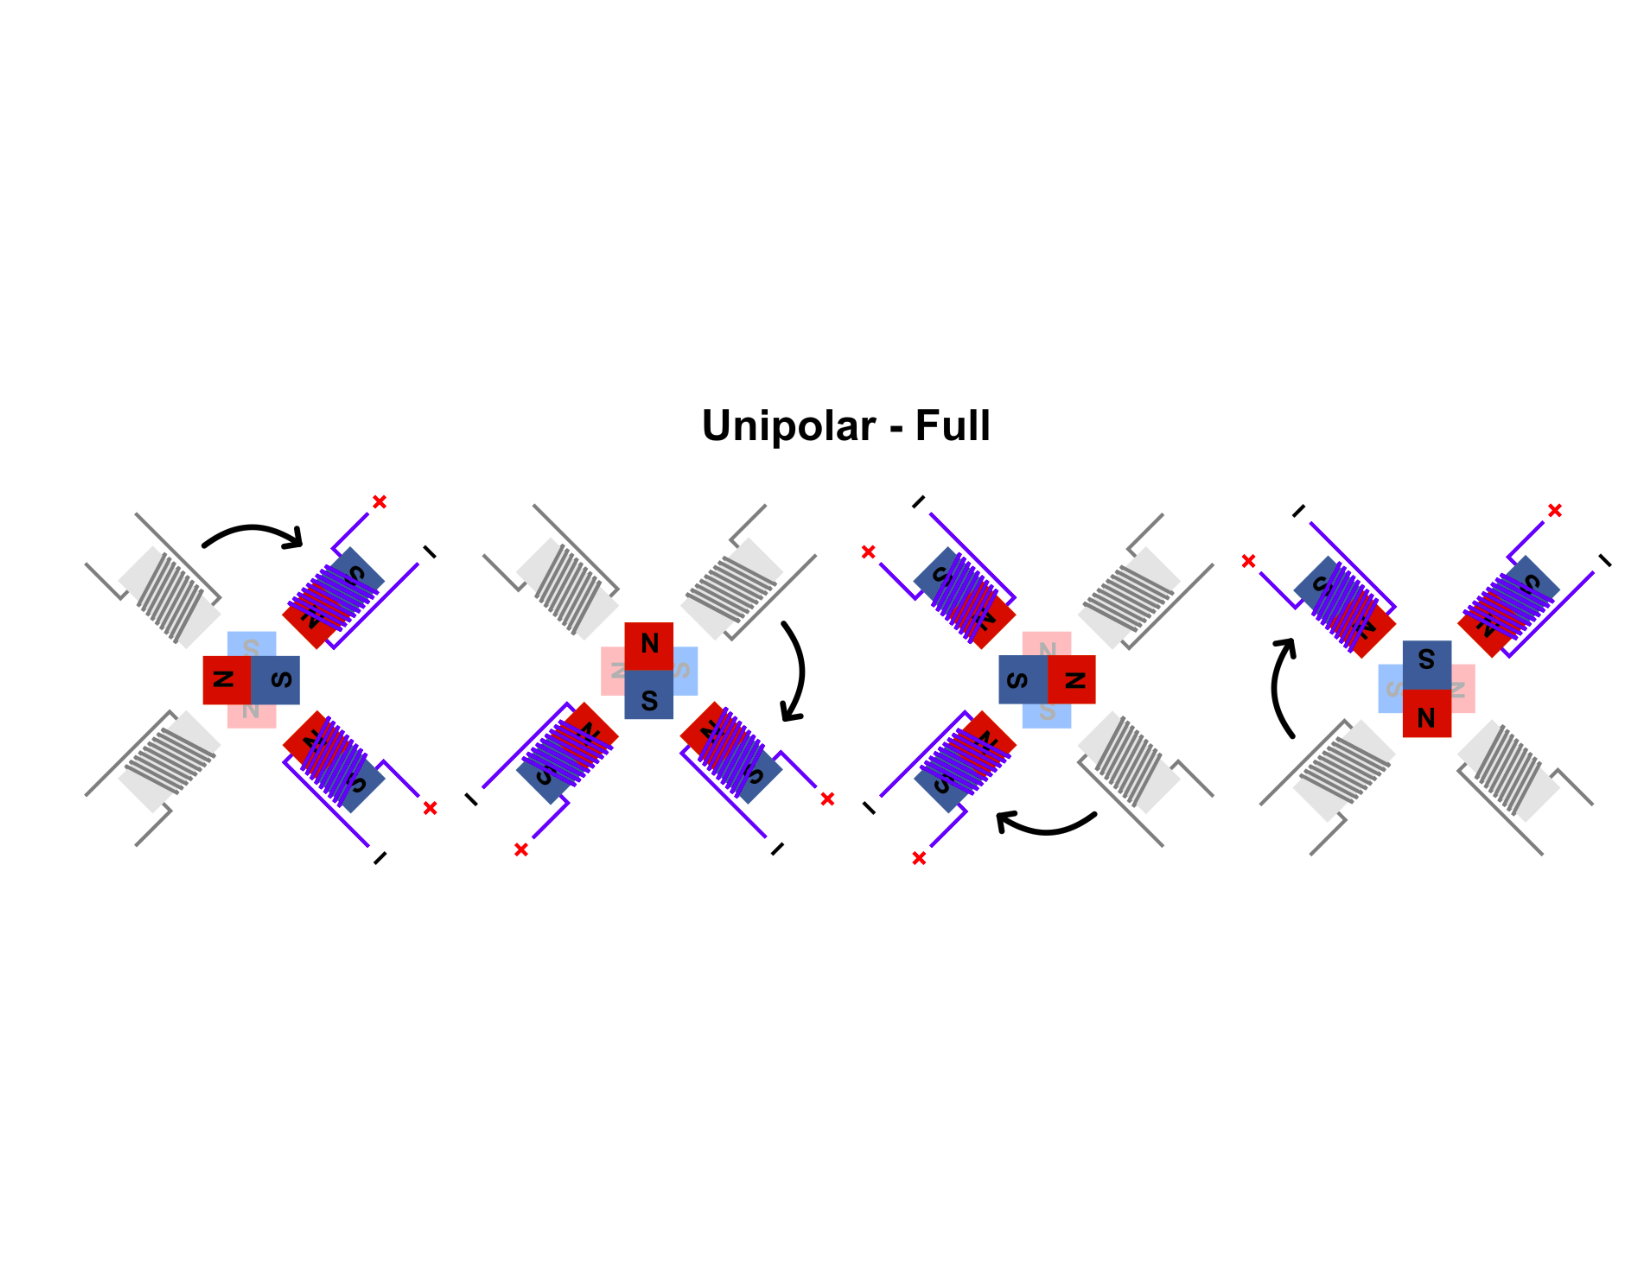
\includegraphics[width=\columnwidth]{images/stepper2.pdf}
  \caption{Working of a steper motor : Full stepping using two coils at a time \cite{stepper2}}\label{f:stepper2}
\end{figure}

With full stepping however, the transition between two consecutive steps is not very smooth. Therefore, a technique called Half stepping is used, where two adjescent coils are turned on similar to full stepping, but between two steps one of the coils is turned off, so that the transition between steps is smooth. This results in a torque 70 percent of that generated in using full stepping with two coils turned on at the same time. This process is shown in figure \ref{f:stepper3} \cite{stepper1}.

\begin{figure}[!ht]
  \centering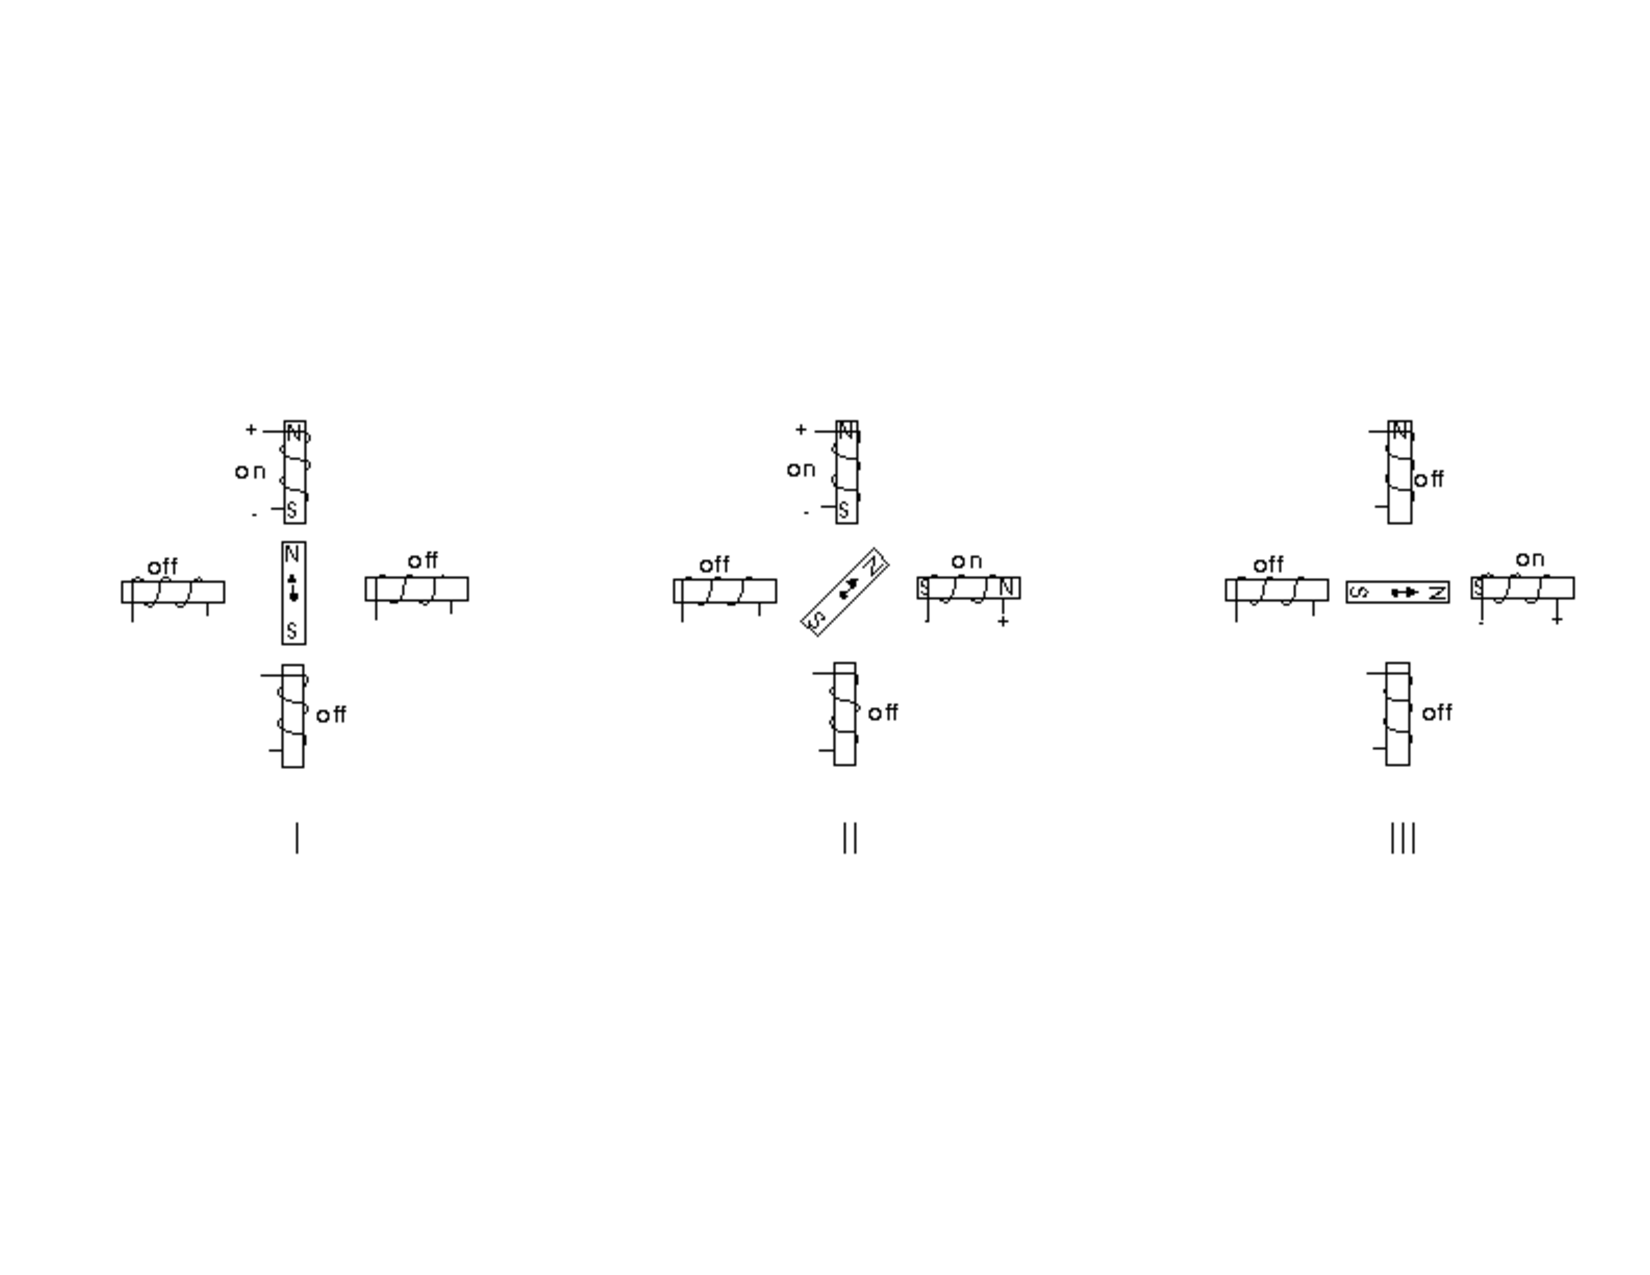
\includegraphics[width=\columnwidth]{images/stepper3.pdf}
  \caption{Working of a steper motor : Half stepping \cite{stepper1}}\label{f:stepper3}
\end{figure}

For this project, the stepper motor 28BYJ-48, provided by Elegoo Industries is used. The motor is driven with the help of a ULN2003 motor driver. The motor is a unipolar steper motor, with a five wire connection to the motor controller and can work with 5 and 12 Volts of DC power supply. When using Half stepping, the step angle of the motor is about 5.625 degrees per step, and when using full stepping the step angle is 11.25 degrees per step.
The motor weighs 30 grams, and a gear ratio of 64:1 \cite{elegoo}\cite{elegoo-desc}.

\subsection{Opencv}

The Open Source Computer Vision library (openCV) is a library of functions aimed at real time computer vision and macine learning and providing a common infrastructure to allow fast progress in the field of computer vision and machine perception \cite{opencv-wiki}\cite{official-opencv}.

The library was originally build by Intel and is now maintained by Itseez and is available freely under open-source BSD License. The library was originally written for C++ but has been developed as cross platform library and supports Python , C++, MATLAB and Java \cite{official-opencv}. for Python the library has been built on top of Numpy, a library that optimizes matrix and vector operations, and takes advantade of MMX and SSE instructions whenever possible. For C++ the library uses the Standart Template Library (STL) as its backbone.

The library has more than 2500 algorithms which include a combination of simple and advanced operations allowing a wide range of operations from edge detection, color detection to object detection, face detection and automatic video stabilization, and motion detection. The opencv-contrib which is an extention to the library built collaboratively by the community contains advanced algorithms that allow processing video in real time \cite{official-opencv}.

OpenCV is widely used in the industry by startups as well as well established organizations like Google, Yhoo, Microdoft, IBM and Intel \cite{official-opencv}.

Opencv can be used to detect faces in real time. The Haar cascades function in the library allows detecting any kind of objects. THe algorithm uses a series of simple classifiers to predict whether a given image has the desired object or not. After training on a large set of positive examples (images containing faces) and negative examples (images not containing faces), the algorithm learns various classifiers, that classify different sections of the image in a manner similar to Adaboost algorithm. Only the portions of the image that are promising are analysed further by more detailed classifiers. This allows the algorithm to run in real time, and detect multiple objects \cite{opencv-haar}\cite{haar-wiki}. Once the classifiers are learned, they can be stored in an XML file which can be used to classify new images. This allows users to obtain XML files available openly for classifiers trained to detect the required object and use them in their programs. Opencv provides XML files for classifiers trained to detect faces and eyes.

The performance of the Haar cascades suffers however, when detecting objects in new images that are present in a different orientation than the ones used to train the classifiers. The classifiers may also fail to differentiate between the object that needs to be detected and similar objects if enough negative examples are not shown while training that include similar objects.

\section{Architecture}

The solution includes two entities the raspberry pi and the desktop, each running two programs. The raspberry pi is connected to the robot car and the raspberry pi can drive the robot car accordig to he message it recieves from the desktop.

There are two programs running on pi, controller\_stepper\_sub.py ans video\_pub.py, and two programs running on the desktop, controller\_pub.py and video\_sub.py.

The programs on both the raspberry pi and the desktop connect to a common broker. the broker may be running on the desktop, or any other place, as long as the IP address of the broker is known. The IP address can be passed as a command line argument when running these programs.

The controller\_pub.py program running on the desktop continuously reads characters from the user and publishes them to the broker under the topic {\em topic/control}. The subsciber controller\_stepper\_sub.py runningon the raspberry pi waits for these messages from the broker and when a message is received it uses the {\em on\_message()} callback to make the robot car move forward, move backward, turn left or turn right, using the half stepping technique described in the previous section.

For monitoring purposes, another program, video\_pub runs on the raspberry pi. This program uses the raspberry pi on board camera with the help of the picamera module and captures images. The images are ocnverted to greyscale, and opencv is used to perform face detection using Haar Cascades. If a face is found, a box is dran around the face in the image. The image is published to the broker under the topic {\em topic/video\_frames}. The video\_sub.py program running on the desktop subscribes to this topic on the broker and displays the images received. These images can be used fo the navigation of the robot car remotely figure \ref{f:arch}.

\begin{figure}[!ht]
  \centering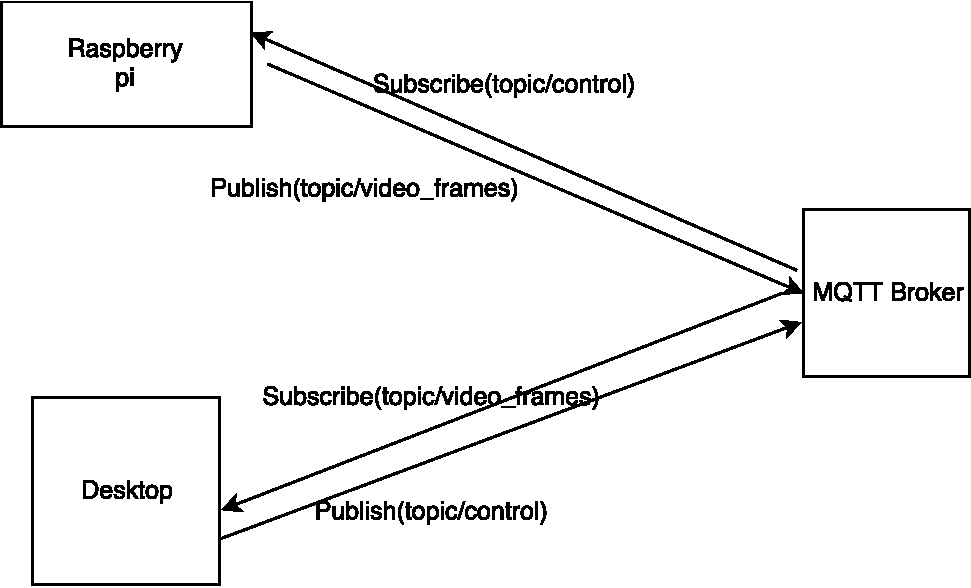
\includegraphics[width=\columnwidth]{images/architecture.pdf}
  \caption{Architecture of the Application}\label{f:arch}
\end{figure}

Using separate programs allow changing the functionality or replacing different parts of the program easily, while keeping the interface same. the program, controller\_sub.py, can be used if contunuous rotation servo motors are used instead of the stepper motors without changing any other part of the application.

The programs can be run easily with the help of a Makefile as described in the next section
\section{Results}
This section covers the setup instructions for the project and the observations.

\subsection{Setup Instructions}

To run the application successfully on both the raspberry pi and the desktop, it must be ensured that all the required libraries are installed. A Makefile has been prvided that can do this on both the raspberry pi and the desktop.

\begin{itemize}

\item First, the motors should be connected to the raspberry pi correctly.
the program uses the raspberr pi GPIO pins , and assumes that for the left motor, the pins IN1, IN2, IN3, IN4 are conected to GPIO pins 7, 11, 13, and 15, and for the right motor, they are connected to GPIO pins, 8, 10, 12, 16, as shown in the connection diagram in figure
\ref{f:connection}

\begin{figure}[!ht]
  \centering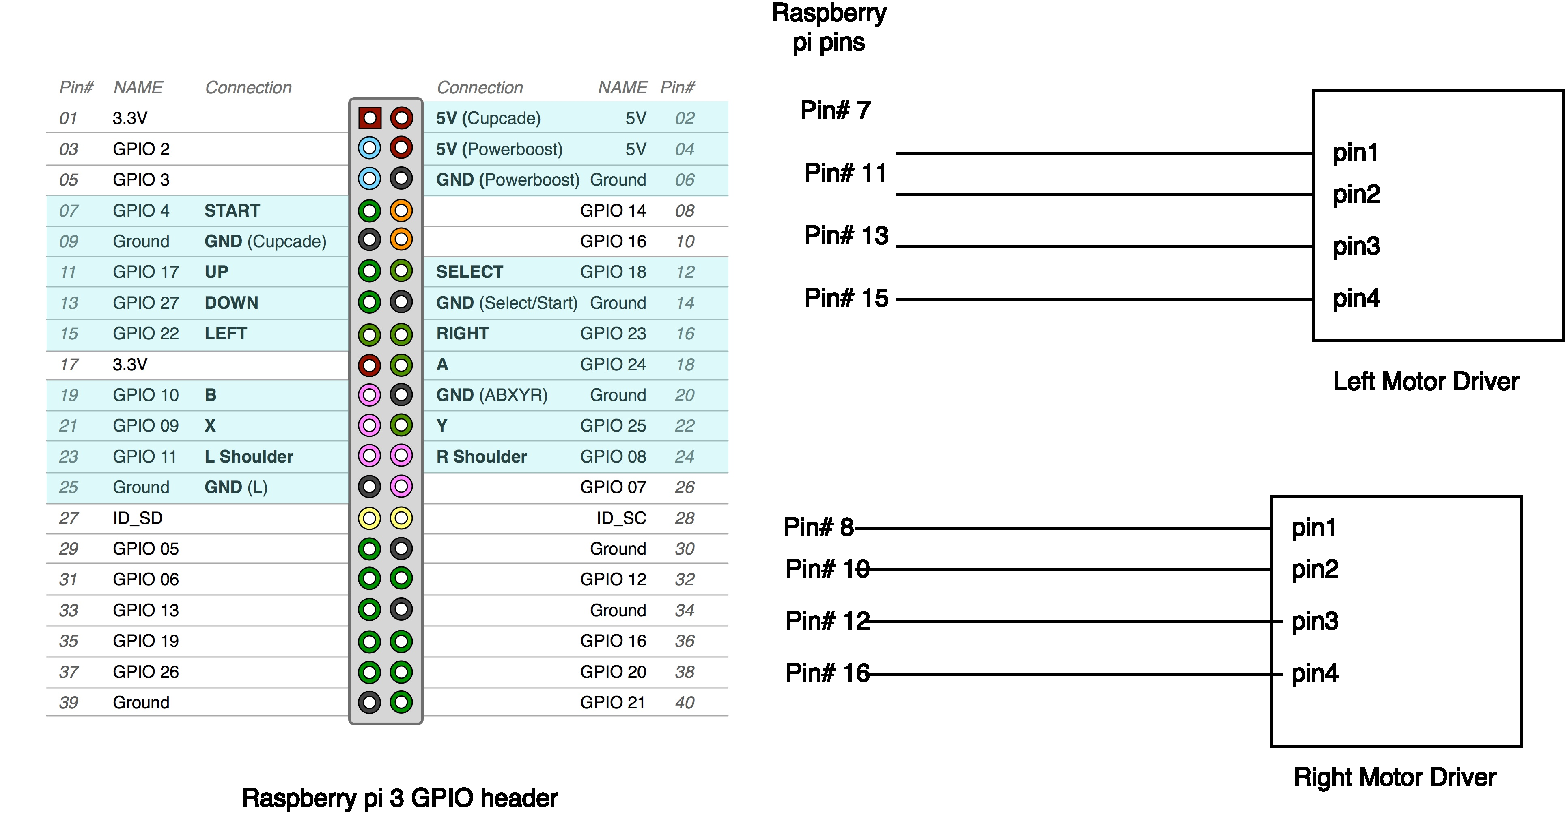
\includegraphics[width=\columnwidth]{images/connection.pdf}
  \caption{Connection Diagram}\label{f:connection}
\end{figure}

\item On the raspberry pi, dependencies for openCV need to be installed. Since the openCV is not available in pip for the arm processor in raspberry pi, we it must be installed from source. This takes a few hours on the raspberry pi. To complete the setup including installation of a MQTT client and opencv on the raspberry pi, clone the repository from github on the raspberry pi and navigate to the code folder, open the terminal and run the command

{\em make setup\_pi}

\item Next, install opencv and an MQTT client and MQTT broker on the desktop. For this, clone the repository from github, navigate into the code folder and run the command 

{\em make setup\_server}

\item Note the IP address of the desktop so that we an connect to the MQTT server running on it. Connect the raspberry pi and the desktop on the same wireless network.

\item To run the code on the desktop, run the command

{\em make run\_server [IP address of the MQTT broker]}

\item Finally to run the code on the raspberry pi, run 

{\em make run\_pi [IP address of the MQTT broker]}

\item Now the raspberry pi car can be controlled by typing in  W, A, S, or D keys on the desktop in the terminal where the program ins running.

\item The program can be stopped on both the raspberry pi and the desktop by running 

{\em make kill}

\end{itemize}

\subsection{Observations}
% how it works on wifi
It was observed that the communication beween the raspberry pi and the desktop controller application is pretty seemless. The robot car responds without any observable delays when the network is strong. When the network is weak, however, some delays may be observed. The delay in becomes more evident in the case of the images sent by the raspberry pi back to the desktop when the network is not strong.

% how motors are jerky sometimes
Using the stepper motors, it is difficult to set a how mush a motor should turn when it recieves a message. If the motor is not allowed to turn long enough, then between two mesages the motor will be idle and if it is turned longe than the interval between two messages, there can be conflicts if in response to each of the messages the subscriber runing on the raspberry pi tries to set a different step on the motor. Therefore, the movement can seem a litle jerky at times.

% how this can be improved using continuos srvo motors
However, this is not a problem with 360 degrees continuous servo motors. Since the continuous servo motors use pulse width modulation, the speed and direction of rotation can be controlled by sending a square wave with different duty cycles depending on the motor. Since, the motor can be stopped and started easily, there are no colflicts even if the motor is allowed to turn longer than the interval between two messages. However, the motor would respond to the two messages one after the other.

Thus the raspberry pi robot car can be successfully controlled over wifi using MQTT for commmunication

\subsection{Improvements}

The project can be improved in various ways. Firstly, even though the deployment with makefile is easy, installing opencv on raspberry pi takes around 4 hours. This can be avoided if we use docker for deployment on the raspberry pi. Two separate images would me needed however one for the processor on the desktop and another one for the arm 8 processor on the raspberry pi.

Machine learning can be incorporated, by collecting the images and the corresponding messages that were sent to the raspberry pi and use it to train a neural network, which could then be used to drive the robot car autonomously. This would be complicated however since car needs to be driven for a long time to get enough data for the neural network to perform well regardless of the surroundings.

Using Haar cascades for face detection leads to a problem that faces can be regognised only if they are resent inthe image in the same orientation as that in the trainig examples. Therefore, it is challenging to recognise all faces in all orientations since it is not possible to train the classifier on images of different faces from all possible angles ans rotations. A better option would be to Concolutional Neural Networks, that help in improving accuracy for the purpose of object detection. Since training and running neural networks may be computationally expensive, it would be a good idea to run it on a server and not on the raspberry pi.

Many diffrent sensors could be added to help improve the monitoring capability of the car, and get more information about the environment.
If many controlling devices and cars are present, the cars may be controlled in groups and other functionality added to behave as a swarm of cars to complete tasks collaboratively.



\section{Conclusion}
MQTT is a fast and reliable data agnostic and platform independent protocol that allows communication between devices. Raspberry pi is small but powerful deveopment board that allows users to build prototypes easily and can be used in various applications because of the significantly powerful arm 8 microprocessor. OpenCv is an open source library for computer vision that is optimised to perform operations on images efficiently and is commonly used in computer vision applications. All these technologies were used to build a robot car, controlled via MQTT over a wireles network. MQTT allows us to easily scale up the number of such cars if needed.

\begin{acks}

  The authors would like to thank Dr. Gregor von Laszewski for giving the opportunity to work on this project and for providign the ncessay ardwawre to complete the project.
  
  The author would also like to thank the associate istructors of th class for their help and for answering questions on piazza which helped everyone.

\end{acks}

\bibliographystyle{ACM-Reference-Format}
\bibliography{report} 

\appendix



\section{Issues}

\DONE{Example of done item: Once you fix an item, change TODO to DONE}

\subsection{Assignment Submission Issues}

    \TODO{Do not make changes to your paper during grading, when your repository should be frozen.}

\subsection{Uncaught Bibliography Errors}

    \TODO{Missing bibliography file generated by JabRef}
    \TODO{Bibtex labels cannot have any spaces, \_ or \& in it}
    \TODO{Citations in text showing as [?]: this means either your report.bib is not up-to-date or there is a spelling error in the label of the item you want to cite, either in report.bib or in report.tex}

\subsection{Formatting}

    \TODO{Incorrect number of keywords or HID and i523 not included in the keywords}
    \TODO{Other formatting issues}

\subsection{Writing Errors}

    \TODO{Errors in title, e.g. capitalization}
    \TODO{Spelling errors}
    \TODO{Are you using {\em a} and {\em the} properly?}
    \TODO{Do not use phrases such as {\em shown in the Figure below}. Instead, use {\em as shown in Figure 3}, when referring to the 3rd figure}
    \TODO{Do not use the word {\em I} instead use {\em we} even if you are the sole author}
    \TODO{Do not use the phrase {\em In this paper/report we show} instead use {\em We show}. It is not important if this is a paper or a report and does not need to be mentioned}
    \TODO{If you want to say {\em and} do not use {\em \&} but use the word {\em and}}
    \TODO{Use a space after . , : }
    \TODO{When using a section command, the section title is not written in all-caps as format does this for you}\begin{verbatim}\section{Introduction} and NOT \section{INTRODUCTION} \end{verbatim}

\subsection{Citation Issues and Plagiarism}

    \TODO{It is your responsibility to make sure no plagiarism occurs. The instructions and resources were given in the class}
    \TODO{Claims made without citations provided}
    \TODO{Need to paraphrase long quotations (whole sentences or longer)}
    \TODO{Need to quote directly cited material}

\subsection{Character Errors}

    \TODO{Erroneous use of quotation marks, i.e. use ``quotes'' , instead of " "}
    \TODO{To emphasize a word, use {\em emphasize} and not ``quote''}
    \TODO{When using the characters \& \# \% \_  put a backslash before them so that they show up correctly}
    \TODO{Pasting and copying from the Web often results in non-ASCII characters to be used in your text, please remove them and replace accordingly. This is the case for quotes, dashes and all the other special characters.}
    \TODO{If you see a figure and not a figure in text you copied from a text that has the fi combined as a single character}

\subsection{Structural Issues}

    \TODO{Acknowledgement section missing}
    \TODO{Incorrect README file}
    \TODO{In case of a class and if you do a multi-author paper, you need to add an appendix describing who did what in the paper}
    \TODO{The paper has less than 2 pages of text, i.e. excluding images, tables and figures}
    \TODO{The paper has more than 6 pages of text, i.e. excluding images, tables and figures}
    \TODO{Do not artificially inflate your paper if you are below the page limit}

\subsection{Details about the Figures and Tables}

    \TODO{Capitalization errors in referring to captions, e.g. Figure 1, Table 2}
    \TODO{Do use {\em label} and {\em ref} to automatically create figure numbers}
    \TODO{Wrong placement of figure caption. They should be on the bottom of the figure}
    \TODO{Wrong placement of table caption. They should be on the top of the table}
    \TODO{Images submitted incorrectly. They should be in native format, e.g. .graffle, .pptx, .png, .jpg}
    \TODO{Do not submit eps images. Instead, convert them to PDF}

    \TODO{The image files must be in a single directory named "images"}
    \TODO{In case there is a powerpoint in the submission, the image must be exported as PDF}
    \TODO{Make the figures large enough so we can read the details. If needed make the figure over two columns}
    \TODO{Do not worry about the figure placement if they are at a different location than you think. Figures are allowed to float. For this class, you should place all figures at the end of the report.}
    \TODO{In case you copied a figure from another paper you need to ask for copyright permission. In case of a class paper, you must include a reference to the original in the caption}
    \TODO{Remove any figure that is not referred to explicitly in the text (As shown in Figure ..)}
    \TODO{Do not use textwidth as a parameter for includegraphics}
    \TODO{Figures should be reasonably sized and often you just need to
  add columnwidth} e.g. \begin{verbatim}/includegraphics[width=\columnwidth]{images/myimage.pdf}\end{verbatim}

re

\end{document}
